% CLASE 1
\label{CLASE1}
\section{Introducción}
\subsection{Distribución de Zona}
\begin{table}[H]
	\centering
	\caption{Zona}
	\begin{tabular}{||c||c|c||}
		\hline
		\hline
		$5$ & Tareas & $45$ \\
		$2$ & Parciales & $30$ \\
		$5$ & Parciales Sorpresa & $5$ \\
		$1$ & Final & $20$ \\
		\hline
		 & Total & $100$ \\
		\hline
		\hline
	\end{tabular}
	\label{zonas}
\end{table}


\subsection{Clases Introductorias}
\subsubsection{Surgimiento de los complejos}

Los números complejos, surgen (en los cursos), a partir de las ecuaciones cuadráticas, tales como:
	$$x^2 + 1 = 0$$
Históricamente, nacen a partir de las ecuaciones cúbicas. \\

Los complejos son un campo, claramente cumple las propiedades de un campo. Además, los complejos forman un espacio vectorial de dimensión $2$ sobre los reales (esto es claro gracias al polinomio minimal). Sabiendo la dimension del EV de los complejos, se escribe un vector cualquiera como combinación lineal de la base, i.e.
	$$z = a+bi$$
Notese que, $\Re{z} = a$ e $\Im{z} = b$, ambas son reales.

% CLASE 2
\label{CLASE2}
\subsubsection{Propiedades Algebraicas de los Complejos}
\paragraph{Conjugados}

El conjugado es el reflejo del número complejo, respecto al eje real. Es decir:
	$$z = a + bi \, \Rightarrow \, \bar{z} = a - bi$$
El signo de la parte imaginaria cambia.


\paragraph{Módulo}

Es el tamaño del vector, es decir, la hipotenusa del triangulo generado por la parte real y la parte imaginaria. Además, el módulo de $z$ es igual al módulo de su conjugado.

\dsnote{Además, se puede encontrar multiplicando el número por su conjugado, i.e. $z\bar{z} = \abs{z} ^2$}


\paragraph{Argumento}

El argumento es el ángulo que hay a partir del eje real positivo. (también es denotado por $\theta$). Esta función esta definida para $\C \setminus \{ 0 \}$. \\

También se tiene que, el argumento es el mismo independientemente de cuantas vueltas se den, es decir:
	$$\text{arg} (z) = \theta + 2k\pi$$
Con $k\in \Z$. De todos estos posibles argumentos, se tiene el \textbf{Argumento Principal}; el cual se define como: el argumento el que esté en el intervalo $(-\pi ,\pi]$, al que denotaremos como:
	$$\text{Arg} (z)$$


\subsubsection{Notación para los Complejos}

\paragraph{Notación Polar o Trigonométrica}

Tomando $\theta = \text{arg} (z)$, se tiene que:
	$$a = \abs{z} \cos{\theta}$$
	$$b = \abs{z} \sin{\theta}$$
Para simplificar la notación se define $\text{cis} \theta = \cos{\theta} + i\sin{\theta}$, con lo que
	$$z = \abs{z} \text{cis} \theta$$

\paragraph{Notación Exponencial o Euleriana}

$$z = \abs{z} e^{i\theta}$$

\dsnote{Más adelante se ahondará más en esta notación.}


\subsubsection{Propiedades}

Propiedades de los números complejos: $z,w\in \C$

\begin{enumerate}[1)]
	\item $\abs{z} = \abs{\bar{z}}$
	\item $z\bar{z} = \abs{z} ^2$
	\item $z + \bar{z} = 2 \Re{z}$
	\item $z - \bar{z} = 2\Im{z} i$
	\item $\Re{z} \leq \abs{z}$
	\item $\Im{z} \leq \abs{z}$
	\item $\bar{\bar{z}} = z$
	\item $\overline{z + w} = \bar{z} + \bar{w}$
	\item $\overline{zw} = \bar{z} \bar{w}$
	\item $\abs{z+w} \leq \abs{z} + \abs{w}$
		\begin{proof}
			Desigualdad Triangular: \\
			\begin{align*}
				\abs{z+w} ^2 &= (z+w)\overline{(z + w)} \\
				&= (z + w)(\bar{z + \bar{w}}) \\
				&= \abs{z} ^2 + \abs{w}^2 + z\bar{w} + \overline{z\bar{w}} \\ 
				&= \abs{z} ^2 + \abs{w}^2 + 2\Re{z\bar{w}} \\
				&\leq \abs{z} ^2 + \abs{w}^2 + 2\abs{z} \abs{\bar{w}} \\
				\abs{z+w} &\leq \abs{z} + \abs{w}
			\end{align*}
		\end{proof}
	\item Si $\abs{z} = 1$, entonces $\bar{z} = \frac{1}{z}$
\end{enumerate}


% CLASE 3
\label{CLASE3}
\subsubsection{El Infinito en los Complejos}

Así como en los reales, existen relaciones de orden, en $\C$ no, no existe una comparación de orden en los números complejos. Esto es más claro analizando la propiedad de tricotomía:
\begin{description}
	\item[$i = 0$] Si la unidad imaginaria fuera cero, entonces no tendría sentido hablar de números imaginarios.
	\item[$i>0$] Si un número es positivo, la desigualdad, al multiplicarla por un positivo, se mantiene. Esto no sucede al multiplicar $i$ (considerandolo positivo) por la desigualdad $i > 0$. Por lo que $i$ no es positivo.
	\item[$i < 0$] Similarmente, con los números negativos. Si se multiplica un número negativo por una desigualdad, esta cambia de "lado". Realizando esto con $i$ (considerandolo negativo) por la desigualdad $i < 0$, se tiene una contradicción. Por lo que, $i$ no es negativo.
\end{description}

Con esto es claro que en los números complejos no hay relaciones de orden. \\

Así como en los reales se tienen dos infinitos (los infinitos no pertenecen a los reales), el negativo y el positivo. En los complejos se tienen inifinos en todas las direcciones, se tienen, infinitos infinitos.

\paragraph{Geometría Proyectiva: } A diferencia de la geometría euclideana, es el postulado de las rectas paralelas. En la geometría proyectiva, dos rectas paralelas si se intersectan. \\

El espacio proyectivo se define como:
	$$\mathbb{P} ^n _\mathbb{K} := \frac{\mathbb{K} \setminus \{ 0 \}}{\sim}$$

Con la relación de equivalencia:
	$$(x_o,\ldots ,x_n) \sim (y_o , \ldots, y_n)$$
	
Si existe $\lambda \neq 0$ tal que
	$$(x_o,\ldots ,x_n) = \lambda (y_o , \ldots, y_n)$$

\subparagraph{Ejemplo: } Tomando $\mathbb{P} ^1 _\R$, es el conjunto de rectas, en $\R ^2$, que pasan por el origen. En general, $\mathbb{P} ^n _\R$, es el conjunto de rectas, $n-$dimensionales, que pasan por el origen. Esto se cumple para más espacios vectoriales.

\dsnote{Se cumple para más espacios vectoriales? Cómo sería algebraicamente?}

Tomando la recta real paralela al eje vertical, es el conjunto que contiene un punto de todas las rectas, excepto del eje vertical. Por lo que:

	$$\mathbb{P} ^1 _\R \cong \R \cup \{ p \} \cong \R \cup \{ \infty \} \cong \text{Circunferencia}$$

Todo es isomorfo a la circunferencia puesto que la circunferencia contiene un punto de todas las rectas, incluyendo la recta "infinito". \\

Para los complejos:
	$$\mathbb{P} ^1 _\C \cong \C \cup \{ \infty \}$$
	

Siguiendo con la idea de la circunferencia, como los complejos "tienen" una dimensión más:
	$$\mathbb{P} ^1 _\C \cong \text{Esfera}$$
	
Esta esfera, es la conocida Esfera de Riemann. Esta esfera es secillo de ver su generación, si se deforma el espacio complejo todo hacia un punto en un eje vertical perpendicular a dicho espacio complejo. 

\begin{figure}[H]
	\centering
	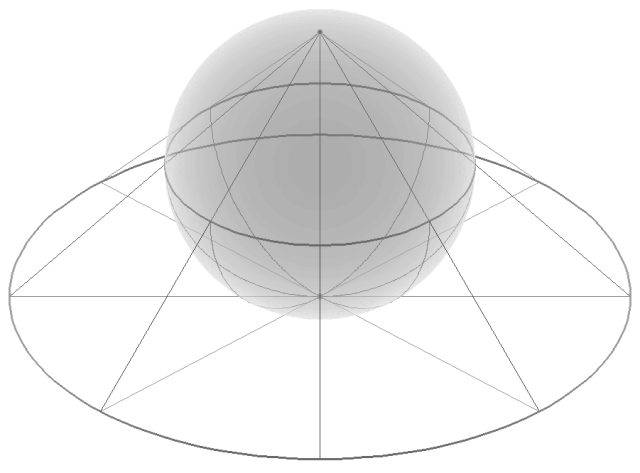
\includegraphics[scale=0.5]{Images/riemannSphere.png}
	\caption{Proyección Estereográfica}
	\label{proy_estereografica}
\end{figure}

Como esta esfera es isomorfa al espacio complejo, existe un isomorfismo entre la esfera y el plano, de modo que todo punto en la esfera tiene asociado un único punto en el espacio complejo.


% CLASE 4
\label{CLASE4}
\subsubsection{Proyección Estereográfica}

Como $\C \cup \{ \infty \} \cong \text{Esfera de Riemann}$, entonces existe un isomorfismo entre ambos espacios. Entonces, a cada punto de la esfera $x_1 ^2 + x_2 ^2 + x_3 ^2 = 1$, se le asocia $z = \flatfrac{(x_1 + ix_2)}{(1 - x_3)}$, es decir: dado $(x_1,x_2,x_3) \in \text{Esfera de Riemann}$
	$$(x_1,x_2,x_3) \mapsto \frac{x_1 + ix_2}{1 - x_3}$$
Para demostrar que dicha transformación es invertible, tomamos el módulo de la parte izquierda:
	$$\abs{z} ^2 = \frac{x_1 ^2 + x_2 ^2}{(1 - x_3)^2}$$
Como dicho punto pertenece a la esfera, entonces se tiene:
	$$ = \frac{1 - x_3 ^2}{(1 - x_3)^2} = \frac{1 + x_3}{1 - x_3}$$
Despejando $x_3$, se tiene:
	$$x_3 = \frac{\abs{z} ^2 - 1}{\abs{z} ^2 + 1}$$
Similarmente, se pueden encontrar expresiones para $x_1$ y $x_2$, con lo que se demuestra que es invertible. Geométricamente, al mapear un punto en la esfera, este punto pertenecerá al plano complejo y a la recta generada por el punto superior de la esfera y el punto de la esfera deseado a mapear.

\paragraph{Ejemplo: } Demostrar que todas las raíces de $p(z) = z^3 + 3z + 5$ tienen módulo mayor a $1$.

\begin{proof}
	Suponiendo que una raíz tiene módulo $\abs{z} \leq 1$, entonces $z^3 + 3z + 5 = 0$, despejando $5$ y enconetrando el módulo de ello se tiene: $\abs{5} = \abs{z^3 + 3z}$ por desigualdad triangular $\abs{z^3 + 3z} \leq \abs{z} ^3 + 3\abs{z}$, por la suposición inicial $\leq 1^3 + 3(1) \leq 4$, lo que es una contradicción, por lo que $\abs{z} > 1$.
\end{proof}
	


% CLASE 5 y 6
\label{CLASE5y6}
\subsection{Teorema de DeMoivre}

Utilizando la notación Eulereana para dos complejos $z,w$, con argumentos $\theta ,\alpha$. Con esto se tiene:
	$$z = \abs{z} e^{i\theta} \quad \quad w = \abs{w} e^{i\alpha}$$
Multiplicando ambos:
	$$zw = \abs{z} \abs{w} e^{i(\theta + \alpha)}$$
Con esta idea, se calcula:
	$$z^n = \abs{z} ^n e^{in\theta}$$
A esto se le conoce como el \textbf{Teorema de DeMoivre}, el cual es cierto, no solo para enteros, sino que para todos los complejos, i.e. $n\in \C$. Esto implica que:
	$$z^n = \abs{z}^n \qty(\cos{n\theta} + i\sin{n\theta})$$

\subsection{Geometría Analítica en $\C$}

\subsubsection{Circunferencia}

Se define como el siguente conjunto:
	$$A = \{ z\in \C : \abs{z} = 1 \}$$
Sin embargo, para una circunferencia desplazada a $z_o$ con radio $r$, se tiene:
	$$\abs{z - z_o} = r$$

\subsubsection{Elipse}

La elipse, asi como en su definición clásica, para sus focos en los puntos $a$ y $b$, se tiene:

	$$\abs{z - a} + \abs{z - b} = k$$
Donde $z$ es todo punto sobre la elipse.

\subsubsection{Recta}

Para una recta entre dos complejos, se tiene que, tomando un parametro $t\in \R$, la recta que pasa por ambos complejos esta dada por:
	$$z + t(z + w)$$
Segmentando dicha recta, se tiene que, para la distancia entre ambos complejos, se limita $t$  a $0 \leq t \leq 1$. Y en base a esto se puede calcular el punto medio entre dos complejos, el cual es simplemente haciendo el valor de $t = 2$.

\subsubsection{Gravicentro}

Sabiendo la relación de las medianas y el gravicentro, entonces tomando los segmentos de recta, simplemente se realiza dicho procedimiento. Tomando cualquier lado (en este caso se tomará $ac$) se tiene que el punto medio entre dichos vértices es:
	$$\frac{a + c}{2}$$
Ahora, para el segmento entre este nuevo punto y el vértice restante es:
	$$b + t\qty(\frac{a + c}{2} - b)$$
Por la relación se tiene que $t = \flatfrac{2}{3}$, con esto y desarrollando se tiene:
	$$\boxed{G = \frac{a + b + c}{3}}$$
	
\dsnote{Ejemplo tarea: \textit{Demostrar que: } $\tan ^2 {1} + \cdots + \tan ^2 {89} \, \in \, \Z$.}



% CLASE 7
\label{CLASE7}
\textbf{Resolviendo el ejemplo: } \\

Tomando la forma polar de un complejo de módulo $1$, se eleva a la $90$ potencia:
	$$\qty(\cos{\alpha} + i\sin{\alpha})^{90} = \cos{90\alpha} + i\sin{90\alpha}$$
Por teorema del Binomio:
	$$\sum _{k=0} ^{90} \binom{90}{k} \cos ^{n - k} {\alpha} \, i^k \sin ^k {\alpha} = \cos{90\alpha} + i\sin{90\alpha}$$
Sabiendo que para potencias pares, la identidad imaginaria es real, entonces:
	$$\sum _{k=0} ^{44} (-1)^k \binom{90}{2k} \cos ^{90 - 2k} {\alpha} \sin ^{2k} {\alpha} = \cos{90\alpha}$$
Reescribiendo el lado izquierdo de la ecuación.

Para $\alpha$ impar:
	$$\sum_{k=0} ^{44} \binom{90}{2k} (-1)^k \tan ^{2k} {\alpha} = 0$$
Entonces, sustituyendo $x = \tan ^2 {\alpha}$, por Cardano$-$Vieta, la suma de todas las soluciones da como resultado uno de los coeficientes del polinomio, por ende, la suma propuesta da como resultado un número entero, por lo que queda demostrado. $\QED$




\section{Funciones Complejas}
Una función compleja, se define igual que las funciones reales, simplemente se tiene que el dominio y el rango son los complejos, es decir:
	$$f:\, \C \to \C$$
En las funciones complejas, no se tienen gráficas como las que se tienen en funciones de $\R$ o $\R^2$. En los complejos, se sabe de, álgebra lineal, que, los complejos son un espacio vectorial de dimensión dos, sobre los reales; de modo que, las funciones son una aplicación de dimension $4$, por lo que no se puede visualizar una gráfica. Para graficar las funciones complejas se toman dos espacios complejos, simplemente para comparar el dominio de la función, con el rango de la misma.

\subsection{Función Exponencial}

Sea $z = x + iy$, se define la exponencial:
	$$e^z := e^x e^{iy}$$
La cual es completamente intuitiva.
	


% CLASE 8
\label{CLASE8}

\subsection{Funciones Seno y Coseno}

Para definir al seno y al coseno, tomamos una forma exponencial:
	$$\sin{z} := \frac{e^{iz} - e^{-iz}}{2i}$$
Y
	$$\cos{z} := \frac{e^{iz} + e^{-iz}}{2}$$

Para la identidad pitagórica, se sabe que se cumple para todo número real; sin embargo, con estas nuevas definiciones, se tiene que dicha identidad es cierta para todo $z\in \C$.

\begin{teorema} \it
	$$\sin ^2 {z} + \cos ^2 {z} = 1$$
\end{teorema}

La demostración es bastante simple, solo se elevan ambas definiciones al cuadrado y por productos notables queda. \\

Además, cumplen todas las identidades ya conocidas para los números reales.
\begin{teorema} \it
	La función:
		$$f(z) = e^{z}$$
	Es periódica, con periodo $2\pi i$
\end{teorema}

Lo curioso de esto, es que la función exponencial para valores reales \textbf{no} es periódica, pero en los complejos si lo es. Para veríficar que la función es periódica simplemente se sustituye la definción de funciones periódicas:
	$$f(z) = f(z + T)$$
La demostración es igual de simple que la anterior, simplemente sustituyendo la definción, se tiene la periodicidad.

\subsubsection{Funciones Seno y Coseno Hiperbólicos}

Para las funciones hiperbólicas, se tienen definiciones muy parecidas a sus respectivas funciones no hiperbólicas, es decir:
	$$\sinh{z} := \frac{e^z - e^{-z}}{2}$$
Y
	$$\cosh{z} := \frac{e^z + e^{-z}}{2}$$
Para todo $z\in \C$.

\subsection{Función Logarítmica}

La función logarítmica debe cumplir ser la inversa de la exponencial, obviamente, en dominio complejo. Entonces, para $z\in \C$, se tiene:
	$$\ln{z} := \ln{\abs{z}} + i\text{arg} (x)$$
Para comprobar que la función logarítmica compleja es, efectivamente, la función inversa de la exponencial. Comprobando con:
	$$f(f^{-1}) = z \quad \quad f^{-1} (f) = z$$
Comprobando que la definción cumple, se tiene:
	$$e^{\ln{z}} = e^{\ln{\abs{z}}} e^{i\text{arg} (z)} = z$$
Ahora, para la otra propiedad de las funciones inversas:
	$$\ln{e^z} = \ln{\abs{e^z}} + i\text{arg} (e^z)$$
Por la forma de la exponencial compleja, se tiene:
	$$= \ln{e^x} + iy = x + iy = z$$
Lo que comprueba las propiedades de función inversa. Cabe recalcar que el logaritmo es una función multivaluada, por lo que se define le logaritmo principal, el cual toma como argumento el argumento principal del complejo. Además, con todo esto, permite encontrar el logaritmo para números negativos. De todo esto, la función logarítmica es válida para $f:\C \setminus \{ 0 \} \to \C$.


% CLASE 9
\label{CLASE9}
\section{Fórmula de Euler}
Tomando $\cos{z} + i\sin{z}$ con $z\in \C$, sustituyendolo por su definición exponencial.
	$$\cos{z} + i\sin{z} = \frac{e^{iz} + e^{-iz}}{2} + i\frac{e^{iz} - e^{-iz}}{2i}$$
Reduciendo, se tiene que:
	$$e^{iz} = \cos{z} + i\sin{z}$$
Para $z\in \C$, esta es la famosa \textbf{Fórmula de Euler}.



% CLASE 10
\label{CLASE10}
\section{Espacios Métricos (Topología de Números Complejos)}

La idea principal de los espacios métricos es la posibilidad de medir distancias.

\begin{definicion} \slshape
	Una función $d:E\times E \to \R$ es una métrica si:
		\begin{enumerate}[a)]
			\item $d(x,y) \geq 0$, para todo $x,y \in E$.
			\item $d(x,y) = 0 \, \Leftrightarrow \, x=y$
			\item $d(x,y) = d(y,x)$ para todo $x,y  \in E$
			\item $d(x,y) \leq d(x,z) + d(z,y)$ para todo $x,y,z\in E$
		\end{enumerate}
\end{definicion}

Si $d:E\times E \to \R$ es una métrica, entonces $(E,d)$ es un espacio métrico. Por ejemplo: 

\begin{itemize}
	\item Tomando $E = \C$ con la métrica definida por el módulo $d(x,y) = \abs{x - y}$, $x,y \in \C$.
	\item Se tiene $E = \C$, para dos elementos del espacio:
		$$d(x,y) = \left\{\begin{array}{cc}
			0 & \text{si } x = y \\
			1 & \text{si } x \neq y
		\end{array}\right.$$
\end{itemize}

\subsection{Proyección Estereográfica}
Tomando un punto en el plano complejo y su respectivo punto en la Esfera de Riemann, la distancia entre dichos dos puntos es:
	$$d(z,z') = \frac{2\abs{z - z'}}{\sqrt{\qty(1 + \abs{z} ^2) \qty(1 + \abs{z'}^2)}}$$
Donde $z$ es el punto en la esfera y $z'$ es el punto sobre el plano complejo.


% CLASE11
\label{CLASE11}
\subsection{Conjuntos Abiertos y Cerrados}

Para iniciar con las definiciones asociadas a ciertos conceptos topológicos, es necesario la base de dichos conceptos, vease, la vecindad, bola, etc. La vecindad se define como:

\begin{definicion} \slshape
	Sea $(E,d)$ un espacio métrico una \textbf{vecindad} centrada en $z_o$ de radio $r>0$ es:
		$$B_r (z_o) := \{ z\in E: d(z_o,z) < r \}$$
	Además, $B$ es vecindad de $w$ si existe $B_r (z_o)$ tal que:
		$$B_r (z_o) \subseteq B$$
\end{definicion}

Con esto, se define:
\begin{definicion} \slshape
	Un conjunto C es \textbf{abierto} si es vecindad de cada uno de sus puntos.
\end{definicion}

\begin{definicion} \slshape
	Un conjunto $C$ es \textbf{cerrado} si $C^c$ es abierto.
\end{definicion}

La definición de conjunto cerrado aparenta ser trivial, sin embargo, la "afirmación": «Un conjunto no es abierto, entonces es cerrado». Puesto que hay conjuntos que son tanto abiertos como cerrados y conjuntos que no son, ni abiertos ni cerrados.



% CLASE12
\label{CLASE12}
\subsection{Sucesiones}

\begin{definicion} \slshape
	Una \textbf{sucesión} de números complejos es una función $f:\N \to \C$. Generalmente representadas como $x_n,(x_n),\ldots$.
\end{definicion}

Ya que se definieron las sucesiones, es lógico pensar en que ciertas sucesiones tienden a ciertos valores, a esto le llamaremos convergencia.

\begin{definicion} \slshape
	Una sucesión $x_n$ \textbf{converge} a un punto $p$ si para cada $\varepsilon > 0$ existe un $N \in \N$ tal que:
		$$d(x_m ,p) < \varepsilon$$
	Si $m > N$.
\end{definicion}

Esta idea induce el siguiente teorema:

\begin{teorema} \it
	Si $x_n$ es convergente, entonces su límite es único
\end{teorema}

\begin{proof}
	Supongamos que $x_n \to p$ y $x_n \to q$. Como $x_n$ convergue a $p$, entonces $\forall \, \varepsilon > 0$ existe $N_1$ tal que:
		$$d(x_m,p) < \frac{\varepsilon}{2} \quad \quad m > N_1$$
	De igual forma, como $x_n \to q$, entonces para todo $\varepsilon > 0$ existe $N_2$ tal que:
		$$d(x_m,q) < \frac{\varepsilon}{2} \quad \quad m > N_2$$
	Por desigualdad triangular
		$$d(p,q) \leq d(x_m ,p) + d(x_m ,q) < \varepsilon \quad \quad \text{si } m > \text{max} \{N_1,N_2 \}$$
	Como se debe de cumplir para todo $\varepsilon > 0$, entonces se tiene $d(p ,q) = 0$ y por definición de métrica se concluye que $p = q$.
\end{proof}

Un teorema más específico para el espacio de los complejos:	

\begin{teorema} \it
	Una sucesión $z_n$ converge a $z = a + bi$ si y solo si
		$$\Re{z_n} \to a$$
	Y
		$$\Im{z_n} \to b$$
\end{teorema}

\dsnote{Se convierte una sucesión de complejos a dos sucesiones independientes de números reales.}


% CLASE 13
\label{CLASE13}
\section{Analiticidad}

\begin{definicion} \slshape
	Una función $f$ es \textbf{derivable} en $z_o \in \C$ si:
		$$\lim _{z\to z_o} \frac{f(z) - f(z_o)}{z - z_o}$$
	existe.
\end{definicion}


\begin{definicion} \slshape
	Una función es \textbf{holomorfa} (analítica) en $z_o$ si es derivable en un abierto que contiene a $z_o$.
\end{definicion}

Al hablar de funciones analíticas recuerda a la definción asociada a series de Taylor, sin embargo, el hecho de que una función compleja es holomorfa, implica directamente que la función sea analítica.

\subsection{Propiedades de las Funciones Holomorfas}
\subsubsection{Teorema de Cauchy$-$Riemann}
\begin{teorema} \it
	Sea $f:\C \to \C$, tal que $f(z) = u(x,y) + iv(x,y)$, donde $z = x + iy$. Entonces si $f$ es holomorfa en $z_o = x_o + iy_o$, entonces
		$$\pdv{x} u(x_o ,y_o) = \pdv{y} v(x_o ,y_o)$$
		$$\pdv{y} u(x_o, y_o) = -\pdv{x} v(x_o ,y_o)$$
	además, $f'(z_o) = u_x (x_o ,y_o) + iv_x (x_o ,y_o)$.
\end{teorema}

Para el converso, si se cumplen las ecuaciones de Cauchy$-$Riemann y las derivadas parciales son continuas, entonces $f$ es holomorfa.

\dsnote{La demostración viene después.}

\begin{ejemplo} \tt
	Demostrar que $f(z) = z^2$ es holomorfa en todos lados y calcular su derivada. \\
	Tomando la función y sustiuyendo $z = x + iy$,
		$$f(z) = (x + iy)^2 = \underbrace{x^2 - y^2}_{u(x,y)} + \underbrace{2xy}_{v(x,y)} i$$
	Es claro que se cumplen las ecuaciones de Cauchy$-$Riemann, además, como las derivadas parciales son continuas para todo $x,y \in \R$, entonces, por el converso del teorema de Cauchy$-$Riemann, la función $f$ es holomorfa. Y la derivada es:
		$$f'(z) = 2x + 2yi = 2z$$
\end{ejemplo}

\begin{definicion} \slshape
	Una función que es holomorfa en todo $\C$ se dice que es \textbf{entera}.
\end{definicion}

\begin{ejemplo} \tt
	Demostrar que $f(z) = e^z$ es entera y calcular su derivada. \\
	
	Separando en parte imaginaria y real:	
		$$f(z) = e^x (\cos{y} + i\sin{y})$$
	En lo que claramente se cumple Cauchy$-$Riemann, y como dichas funciones son continuas en todos los puntos, por lo que, la función es entera. Entonces, la derivada es:
		$$f'(z) = e^x (\cos{y} + i\sin{y}) = e^z$$
\end{ejemplo}

\begin{ejemplo} \tt
	Demostrar que $f(z) = \bar{z}$ no es holomorfa en ningún lado. \\
	Realizando Cauchy$-$Riemann, no se cumple la primera encuación $C-R$. Entonces no es holomorfa en ningún lado. Por lo que dicha función no es derivable.
\end{ejemplo}


% CLASE 15
\label{CLASE15}
\subsubsection{Teorema de la Función Inversa Versión Compleja}
\begin{teorema} \it
	Si $f$ es holomorfa y $f'(z_o) \neq 0$, entonces existe un abierto que contiene a $z_o$ tal que
		$$\dv{w} f^{-1} (w) = \frac{1}{f'(z)}$$
	en donde $w=f(z)$, para $z$ en el abierto.
\end{teorema}

\begin{ejemplo} \tt
	Si $f$ es una función holomorfa, entonces las curvas de nivel de sus partes real e imaginaria son perpendiculares entre si. \\
	Por definición de gradiente, se tiene que:
		$$\langle \grad{u} ,\grad{v} \rangle = u_x v_x + u_y v_y$$
	Por Cauchy$-$Riemann, entonces:
		$$\langle \grad{u} ,\grad{v} \rangle = 0$$
	Lo que los gradientes, se intersectan perpendicularmente, entonces las curvas de nivel se intersectan perpendicularmente. $\QED$
\end{ejemplo}


% CLASE 16
\label{CLASE16}
\subsubsection{Funciones Armónicas}

\begin{definicion} \slshape
	Una función $\phi :\R ^2 \to \R$ es \textbf{armónica} si
		$$\nabla ^2 \phi = 0$$
\end{definicion}



\begin{teorema} \it
	Las partes real e imaginaria de una función holomorfa son armónicas.
\end{teorema}

\begin{proof}
	Sean $f(z) = u(x,y) + iv(x,y)$ una función holomorfa. Entonces, satisface las ecuaciones de Cauchu$-$Riemann:
		$$u_x = v_y \quad \quad u_y = - v_x$$
	Derivando otra vez las ecuaciones de C$-$R y, utilizando el teorema de Cairaut, derivando respecto a $x$, se tiene:
		$$u_{xx} + u_{yy} = v_{xy} - v_{yx} = 0$$
	Similarmente, $v$ es armónica.
\end{proof}


\begin{definicion} \slshape
	Sea $u$ una función armónica. Una función $v: \R^2 \to \R$ que hace que la función:
		$$f(z) = u + iv$$
	sea holomorfa, se le llama \textbf{Conjugado Armónico} de $u$.
\end{definicion}



\subsection{Demostración Teorema Cauchy$-$Riemann}
Tomando la definición compleja de derivada:
	$$f'(z_o) = \lim_{\Delta z \to 0} \frac{f(z_o + \Delta z) - f(z_o)}{\Delta z}$$
Sabiendo que para determinar la existencia de un límite de una función compleja (siguiendo la idea del calculo multivariable), es necesario que desde cualquier trayectoria, hacia el punto en concreto el límite tenga el mismo valor. Por lo que, reescribiendo el límite:
	$$ = \lim _{\Delta z \to 0} = \frac{u(x_o + \Delta x, y_o + \Delta y) + iv(x_o + \Delta x, y_o + \Delta y) - u(x_o,y_o) - v(x_o,y_o)}{\Delta x +i\Delta y}$$
	
Tomando dos formas para aproximarse al cero, de este nuevo límite, es, primero, aproximando por el eje real.
	
	$$ = \lim _{\Delta x \to 0} \frac{u(x_o + \Delta x, y_o) - u(x_o,y_o)}{\Delta x} + i\lim _{\Delta x \to 0} \frac{v(x_o + \Delta x, y_o) - v(x_o,y_o)}{\Delta x} = \pdv{u}{x} (x_o,y_o) + i\pdv{v}{x} (x_o,y_o)$$
La segunda forma, es por medio del eje imaginario:
	$$\lim _{\Delta y \to 0} \frac{u(x_o, y_o + \Delta y) - u(x_o,y_o)}{i\Delta y} + i\lim _{\Delta x \to 0} \frac{v(x_o, y_o + \Delta y) - v(x_o,y_o)}{i\Delta y} = -i\pdv{u}{y} (x_o,y_o) + \pdv{v}{y} (x_o,y_o)$$

Como $f'(z_o)$ existe, se sabe que todoslos caminos diferentes para aproximar $\Delta z\to 0$ deben ser iguales; de modo que, igualando parte real y parte imaginaria se tiene:
	$$\pdv{u}{x} = \pdv{v}{y} \quad \quad \pdv{u}{y} = -\pdv{v}{x}$$
$\QED$

% CLASE 14
\label{CLASE14}
\section{Límites en Funciones Complejas}

Se define límite para una función definida de $f:\C \to \C$:

\begin{definicion} \slshape
	Sea $f$ definida en un conjunto que contiene alguna vecindad de radio $r$ centrada en $z_o$. Se dice que el límite cuando $z$ tiende a $z_o$ de $f(z)$ es $w$, el cual se denota por:
		$$\lim _{z\to z_o} f(z) = w$$
	si para cada $\varepsilon > 0$, existe $\delta > 0$ tal que para todo $z\neq z_o$ en $V_r (z_o)$, se cumple que
		$$\abs{f(z) - w} < \varepsilon$$
	Siempre que $\abs{z - z_o} < \delta$.
\end{definicion}

\begin{teorema} \it
	El límite de una función compleja es \textbf{único}, si es que existe.
\end{teorema}

\begin{proof}
	Supongamos que:
		$$\lim _{z\to z_o} f(z) = a$$
	Y 
		$$\lim _{z\to z_o} f(z) = b$$
	con $a\neq b$ y, sea $\varepsilon = \flatfrac{\abs{a - b}}{2} > 0$. Por definición de límite, sea $\delta > 0$ tal que $\abs{z - z_o} <\delta$ implica que $\abs{f(z) - a} < \varepsilon$ y $\abs{f(z) - b} < \varepsilon$.
	Entonces:
		$$\abs{a - b} \leq \abs{a - f(z)} + \abs{f(z) - b} < 2\varepsilon$$
	Lo que claramente es una contradicción, entonces $a\neq b$.
\end{proof}

Lo interesante es que para funciones de variable compleja, las propiedades de los límites (álgebra de los límites) sigue siendo igual, por lo que no se ahondará en ello.

\begin{ejemplo} \tt
	Determinar si el límite existe:
		$$\lim _{z\to 0} \qty(\frac{z}{\bar{z}}) ^2$$
	Como en varias variables, para que un límite exista, es necesario que de el mismo valor desde todas sus trayectorias, por lo que, es más sencillo determinar la no existencia del límite; de modo que, acercandolos por la trayectoria sobre el eje real:
		$$\lim _{z\to 0} \qty(\frac{x}{x})^2 = 1$$
	Y por la recta $y=x$:
		$$\lim _{z\to 0} \qty(\frac{x + xi}{x - xi}) ^2$$
	Luego de un poco de desarrollo algebraico, se tiene que dicho límite es igual a:
		$$\lim _{z\to 0} \qty(\frac{x + xi}{x - xi}) ^2 = e^{i\pi} = -1$$
	Por lo que el límite no existe.
\end{ejemplo}

\subsection{Continuidad}

\begin{definicion} \slshape
	Una funcion compleja $f$ es continua en $z_o$ si su límite existe y:
		$$\lim _{z\to z_o} f(z) = f(z_o)$$
\end{definicion}





\begin{definicion}
	Una función $\phi :\R ^2 \to \R$ es \textbf{armónica} si
		$$\nabla ^2 \phi = 0$$
\end{definicion}



\begin{teorema}
	Las partes real e imaginaria de una función holomorfa son armónicas.
\end{teorema}

\begin{proof}
	Sean $f(z) = u(x,y) + iv(x,y)$ una función holomorfa. Entonces, satisface las ecuaciones de Cauchu$-$Riemann:
		$$u_x = v_y \quad \quad u_y = - v_x$$
	Derivando otra vez las ecuaciones de C$-$R y, utilizando el teorema de Cairaut, derivando respecto a $x$, se tiene:
		$$u_{xx} + u_{yy} = v_{xy} - v_{yx} = 0$$
	Similarmente, $v$ es armónica.
\end{proof}



\begin{lema} \it
	Si $f$ es una función diferenciable en $z_o$, entonces $f$ es continua en $z_o$.
\end{lema}


















































